\documentclass[11pt, oneside]{article}
%
%   get various packages
%
\usepackage[margin=1.0in]{geometry}                                     % adjust margins
\geometry{letterpaper}                                                  % ... or a4paper or a5paper or ... 
\usepackage{url}                                                        % need this to use URLs in bibtex
\usepackage{setspace}                                                   % need this for \setstrech{...}
\usepackage{scrextend}                                                  % need this for addmargin
\usepackage[export]{adjustbox}                                          % need this to get frame for includegraphics
\usepackage{bigints}                                                    % bigger integral symbol
%
%   tikz et al
%
\usepackage{tikz}
\usetikzlibrary{calc,patterns,angles,quotes,shapes,math,decorations,
                through,intersections,lindenmayersystems,backgrounds}    
\usepackage{pgfplots}
\usepackage{pgfplots}	
%
%	math stuff
%
\usepackage{amsmath,amsfonts,amssymb,amsthm}
\usepackage{mathtools}
\usepackage{commath}                                                    % get \norm{x}
\usepackage{fixmath}                                                    % get \mathbold
\usepackage{gensymb}                                                    % get \degree
\usepackage{circuitikz}                                                 % draw circuits
\usepackage{mathrsfs}

\usepackage{hyperref}
\usepackage{url}
\usepackage{subcaption}
\usepackage{authblk}
\usepackage{amsmath}
\usepackage{mathtools}
\usepackage{graphicx}
\usepackage[export]{adjustbox}
\usepackage{hyperref}
\usepackage{alltt}
\usepackage{color}
\usepackage[utf8]{inputenc}
\usepackage[english]{babel}
\usepackage{float}
\usepackage{bigints}
\usepackage{braket}
\usepackage{siunitx}
\usepackage{relsize}
\usepackage{multirow}
\usepackage{esvect}



%
%	watermarks
%
% \usepackage{draftwatermark}
% \SetWatermarkText{Draft}
% \SetWatermarkScale{5}
% \SetWatermarkLightness {0.9} 
% \SetWatermarkColor[rgb]{0.7,0,0}
%
%
\theoremstyle{definition}
\newtheorem{theorem}{Theorem}[section]
\newtheorem{definition}{Definition}[section]
\newtheorem{proposition}{Proposition}[section]
\newtheorem{lemma}{Lemma}[section]
\newtheorem{example}{Example}[section]
\newtheorem{remark}{Remark}[section]
%
%
%	so you can do e.g., \begin{bmatrix}[r] (or [c] or [l])
%
%
\makeatletter
\renewcommand*\env@matrix[1][c]{\hskip -\arraycolsep
  \let\@ifnextchar\new@ifnextchar
  \array{*\c@MaxMatrixCols #1}}
\makeatother
%
%
%
\newcommand{\argmax}{\operatornamewithlimits{argmax}}
\newcommand{\argmin}{\operatornamewithlimits{argmin}}
%
%	handy command
%
\newcommand*{\Scale}[2][4]{\scalebox{#1}{$#2$}}%
%
%
%
\title{Notes on Attention Models for Neural Networks}
\author{David Meyer \\ dmm613@gmail.com}
\date{Last update: \today}


\begin{document}
\maketitle

\section{Introduction} 
\label{sec:intro}
Statistical language models are probability distributions which
have many applications, including speech recognition, machine
translation, part-of-speech tagging, parsing, handwriting
recognition, and information retrieval. Given a sequence
of length $n$, a language model assigns a probability
$p(x_{1},\ldots ,x_{n})$ to the whole sequence.  Here $x_i$ is
the $i^{th}$ word or symbol in the sequence.  A model that
computes either $p(x_{1},\ldots ,x_{m})$ or $p(x_{n} | x_1, x_2,
\cdots, x_{n-1})$ is called a language model. Using the chain
rule for conditional 
probabilities \cite{chain_rule_for_conditional_probabilities}, 
we can see that

\begin{flalign}
\label{eqn:chain_rule}
p(x_{1}, x_{2}, \ldots, x_{n}) &= p(x_{1}) p(x_{2} | x_{1})
p(x_{3} | x_{1}, x_{2}) \cdots p(x_{n} | x_{1}, \ldots, x_{n -
1}) \\
\label{eqn:chain_rule_prod}
&= \prod\limits_{i = 1}^{n} p(x_{i} | x_{1}, x_{2}, \ldots, x_{i - 1})
\end{flalign}


\noindent
Observe that since our language model is
sequential\footnote{$x_i$ occurs before $x_j$ $\forall {i,j} \; 1
\leq i < j$}, the value of $n$ in Equation
(\ref{eqn:chain_rule_prod}) is in some sense how far back in time
we need to look to predict the next word or symbol (I'll just say
word from here on out). A language model that looks at the $n$
previous words in a sequence is called an \emph{n-gram}, and is
defined using the chain rule as shown in Equation
(\ref{eqn:chain_rule}). Interesting n-gram models include

\begin{equation*}
\begin{array}{lllll}
p(x_{1},x_{2},\ldots,x_{n}) 
	&\approx& \prod\limits_{i = 1}^{n} p(x_{i}) 
	&\qquad \mathbin{\#} \text{ the unigram model} \\
p(x_{i} | x_{1},x_{2},\ldots, x_{i -1}) 
	&\approx& p(x_{i} |  x_{i-1})   
	&\qquad \mathbin{\#} \text{ the bigram model}
\end{array}
\end{equation*}


\bigskip
\noindent
The unigram model assumes we can predict the $i^{th}$ word, 
$x_i$, independently of $x_1,x_2,\hdots,x_{i-1}$ (the words 
that came before it). The bigram model assumes that the 
future is independent of the past given the present, 
i.e., the Markov assumption.\footnote{Sometimes called a 
first-order Markov assumption.}

\bigskip
\noindent
Note that we can estimate the n-gram probabilities in a
straightforward way. Consider the bigram case. Here the
Maximum Likelihood Estimate (MLE) is simply is


\begin{equation*}
\begin{array}{llll}
p(x_{i} |x_{i-1}) 
	&=& \dfrac{\text{count}(x_{i-i}, x_{i})}{\text{count}(x_{i-1})}
    &\qquad \qquad \qquad \mathbin{\#} \text{ bigram MLE estimate}
\end{array}
\end{equation*}

\bigskip
\noindent
Here we are simply counting how many times $x_{i}$ appeared in
the context $x_{i-1}$ and normalizing by all observations of
$x_{i-1}$. 

\bigskip
\noindent
There are a few problems with \emph{n-gram} models. First, for
any reasonable $n$ the \emph{n-gram} is likely to be an
insufficient model of the language due to the long-range dependencies
typically found in natural language.  This forces larger values
of $n$. The second is that \emph{n-grams} suffer from sparse data
distributions; as $n$ grows the space of all possible sequences
grows rapidly and the probability of most sequences or next words
is tends towards zero. In addition, the number of possible
parameters grows exponentially with $n$. As a result, there will
be never enough of the training data to estimate parameters of
high-order \emph{n-gram} models. That said, there are many cases
in which we can get away with \emph{n-grams}.

\section{Encoder-Decoder Architecture}
\noindent
Recurrent Neural Networks (RNNs) take a different approach to
machine translation. Rather than keeping counts, a RNN summarizes
what it has seen previous steps in its current hidden state; you
can think of the hidden state $h_t$ as the memory of the
network. Thus $h_t$ captures information about what happened in
the previous $t-1$ time steps. This means that the RNN must be
able to summarize all the information from the $t-1$ previous
steps in a \emph{fixed length} vector ($h_t$). This property will
turn out to be one of the limitations of RNNs that motivated the
development of attention mechanisms. Finally, note that the
output distribution at time $t$, $y_t$, s calculated solely based
on $h_t$.

\bigskip
\noindent
As an aside, while a vanilla RNNs can in principle capture
dependencies over some period of time in past, in practice they
have trouble with long-range dependencies. As a result, these
networks are typically outfitted with some kind of memory, such
as in the Long Short-Term Memory (LSTM) or the gated units
described in \cite{Cho:2014aa}. Note here: Neural Turing Machines
\cite{Graves:2014aa} and Differentiable Neural Computers
\cite{Graves:2016aa} use a more explicit and function memory;
however, as pointed out in \cite{Daniluk:2017aa} the hidden state
matrix is just a memory matrix of the form $[h_{t-L}\ldots
h_{t-1}] \in \mathbb{R}^{n \times L}$, where $n$ is the output
dimension of the RNN cells and $L$ is a sliding window.


\bigskip
\noindent
Recent state of the art performance on translation tasks has
been achieved using the Encoder-Decoder framework as described 
in Sutskever et al. \cite{NIPS2014_5346} and Cho
et al. \cite{Cho:2014aa}. The following description of the
Encoder-Decoder framework follows the notation found in
\cite{Bahdanau:2014aa}.

\bigskip
\noindent
In the Encoder-Decoder framework, an encoder reads the input
sentence, which is a sequence of vectors $\mathbf{x} = (x_1,
\cdots, x_{T_x})$.  The input sequence is taken from a vocabulary
$V_x$, with $|V_x| = K_x$. Here each $x_i$ is a column vector of
length $K_x$ such that $x_i \in \mathbb{R}^{K_{x} \times 1}$
(usually written $x_i \in \mathbb{R}^{K_x}$) is the one-hot
encoding for the word at position $i$. That is, the $i^{th}$
input word looks like

\begin{flalign*}
x_i = \begin{bmatrix}
x_{1i} \\
x_{2i} \\
\vdots \\
x_{K_{x}i} 
\end{bmatrix}
\end{flalign*}

\bigskip
\noindent
so that

\bigskip

\begin{flalign*}
\mathbf{x} = \begin{bmatrix}
x_{11} & x_{12} & \cdots & x_{1i} & \cdots & x_{1T_x} \\
x_{21} & x_{22} & \cdots & x_{2i} & \cdots & x_{2T_x}\\
\vdots & \vdots & \ddots & \vdots & \ddots  & \vdots\\
x_{K_{x}1} & x_{K_{x}2} & \cdots & x_{K_{x}i} & \cdots &  x_{K_{x}T_x} \\
\end{bmatrix} 
\end{flalign*}

\bigskip
\noindent
The encoder RNN calculates its hidden state\footnote{In general
the hidden state of the encoder is called $h_t$ and the hidden
state of the decoder is called $s_t$.} at time $t$, $h_t \in
\mathbb{R}^n$ as

\begin{flalign*}
\label{eqn:h_sub_t}
h_t = f(x_{t},h_{t-1})
\end{flalign*}

\bigskip
\noindent
and also produces a context vector $c$ from the hidden states: $c
= q(\{h_{1},h_{2},\ldots, h_{T_x}\})$.  As an example,
\cite{NIPS2014_5346} used an LSTM for $f$ and defined
$q(\{h_{1},h_{2},\ldots, h_{T}\}) = h_{T}$.

\bigskip
\noindent
The decoder is usually trained to predict the next word $y_t$
given the context vector $c$ and all the previously predicted
words $\{y_1, \ldots, y_{t-1}\}$; the decoder defines a
probability over $\mathbf{y}$ (the translation) by decomposing it
into its joint probabilities, conditioned on the previously
translated words and the context vector.

\begin{flalign*}
p(\mathbf{y}) = \prod\limits_{t = 1}^{T} p(y_{t} |\{ y_{1}, y_{2}, 
\ldots, y_{T_y}\},c)
\end{flalign*}

\bigskip
\noindent
where $\mathbf{y} = (y_{1},\ldots,y_{T_y})$. With an RNN, the
conditional probability of each translation is modeled as

\begin{flalign*}
p(y_{t} |\{ y_{1}, y_{2}, \ldots, y_{T_y}\},c) = g(y_{t-1}, s_t,c)
\end{flalign*}

\bigskip
\noindent
where $g$ is a nonlinear, potentially multi-layered, function
that outputs the probability of $y_t$, and $s_t$ is the hidden
state of the RNN.

\bigskip
\noindent
Recurrent Neural Networks (RNNs) take a different approach to
machine translation.  From a probabilistic perspective, the
machine translation task is to find a target sentence \textbf{y}
that maximizes the conditional probability of \textbf{y} given a
source sentence \textbf{x}, that is, $\argmax
p(\mathbf{y} | \mathbf{x})$ (where the $\argmax$ is over \textbf{y}). 
In neural machine translation, a
parameterized model is fit which maximizes the conditional
probability of sentence pairs using a parallel training corpus.



\subsection{Preliminaries}
\noindent
We consider an input sequence over a vocabulary $V_x$, with
$|V_x| = K_x$, where the input is a sequence of vectors
$\mathbf{x} = (x_1, \cdots, x_{T_x})$. Here each $x_i$ is a
column vector of length $K_x$ such that $x_i \in
\mathbb{R}^{K_{x} \times 1}$ (usually written $x_i \in
\mathbb{R}^{K_x}$) is the one-hot encoding for the word at
position $i$. That is, the $i^{th}$ input word looks like

\bigskip
$x_i = \begin{bmatrix}
x_{1i} \\
x_{2i} \\
\vdots \\
x_{K_{x}i} 
\end{bmatrix}$

\bigskip
\noindent
so that

\bigskip
$\mathbf{x} = \begin{bmatrix}
x_{11} & x_{12} & \cdots & x_{1i} & \cdots & x_{1T_x} \\
x_{21} & x_{22} & \cdots & x_{2i} & \cdots & x_{2T_x}\\
\vdots & \vdots & \ddots & \vdots & \ddots  & \vdots\\
x_{K_{x}1} & x_{K_{x}2} & \cdots & x_{K_{x}i} & \cdots &  x_{K_{x}T_x}
\end{bmatrix}
$

\section{RNN Encode-Decoder Architecture} 
\label{sec:rnn}

\section{Appendix A: The Evolution of Attention Models}
\label{sec:appendix_a}

\begin{figure}[H]
\center{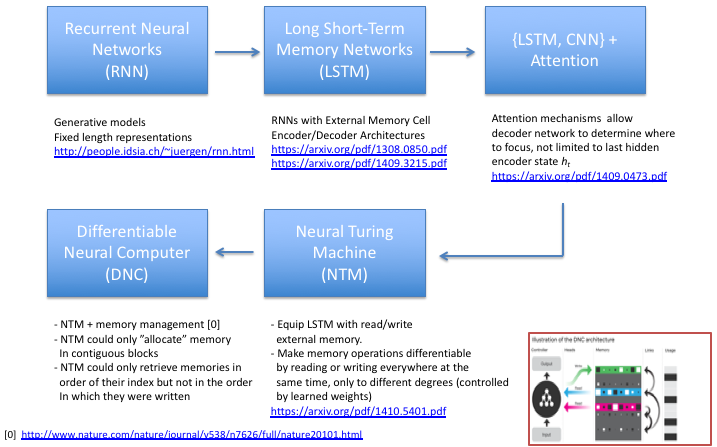
\includegraphics[cfbox=black,scale=0.65]
       {images/attention_evolution.cropped.png}}
\caption{The Evolution of Attention Models}
\label{fig:attention_evolution}
\end{figure}
%
%
%
\section*{Acknowledgements}
Thanks to Stephen Wolff for pointing out Shannon's work 
in this area \cite{shannon_thesis,the_shannonizer}.
%
%	LaTeX source on overleaf.com
%
\section*{\LaTeX \hspace{0.10 mm} Source}
\url{https://www.overleaf.com/read/gshqdkhqdnmm}
%
%	get a bibliography
%
%	Note:.bib files go in ~/Library/texmf/bibtex/bib with TeXShop (MacTeX).
%	You can also use an absolute path, e.g. \bibliography{/Users/dmm/papers/bib/qc}
%
\bibliographystyle{plain}
\bibliography{ml}
%
%	done
%
\end{document} 

